% mnras_template.tex
%
% LaTeX template for creating an MNRAS paper
%
% v3.0 released 14 May 2015
% (version numbers match those of mnras.cls)
%
% Copyright (C) Royal Astronomical Society 2015
% Authors:
% Keith T. Smith (Royal Astronomical Society)

% Change log
%
% v3.0 May 2015
%    Renamed to match the new package name
%    Version number matches mnras.cls
%    A few minor tweaks to wording
% v1.0 September 2013
%    Beta testing only - never publicly released
%    First version: a simple (ish) template for creating an MNRAS paper

%%%%%%%%%%%%%%%%%%%%%%%%%%%%%%%%%%%%%%%%%%%%%%%%%%
% Basic setup. Most papers should leave these options alone.
\documentclass[a4paper,fleqn,usenatbib]{mnras}

% MNRAS is set in Times font. If you don't have this installed (most LaTeX
% installations will be fine) or prefer the old Computer Modern fonts, comment
% out the following line
\usepackage{newtxtext,newtxmath}
% Depending on your LaTeX fonts installation, you might get better results with one of these:
%\usepackage{mathptmx}
%\usepackage{txfonts}

% Use vector fonts, so it zooms properly in on-screen viewing software
% Don't change these lines unless you know what you are doing
\usepackage[T1]{fontenc}
\usepackage{ae,aecompl}


%%%%% AUTHORS - PLACE YOUR OWN PACKAGES HERE %%%%%

% Only include extra packages if you really need them. Common packages are:
\usepackage{graphicx}	% Including figure files
\usepackage{amsmath}	% Advanced maths commands
\usepackage{amssymb}	% Extra maths symbols
\usepackage[dvipsnames]{xcolor}
%%%%%%%%%%%%%%%%%%%%%%%%%%%%%%%%%%%%%%%%%%%%%%%%%%

%%%%% AUTHORS - PLACE YOUR OWN COMMANDS HERE %%%%%

% Please keep new commands to a minimum, and use \newcommand not \def to avoid
% overwriting existing commands. Example:
%\newcommand{\pcm}{\,cm$^{-2}$}	% per cm-squared
\newcommand{\angus}[1]{\color{JungleGreen}#1\color{black}}
\newcommand{\chris}[1]{\color{orange}#1\color{black}}
\newcommand{\marksul}[1]{\color{red}#1\color{black}}
\newcommand{\maria}[1]{\color{RubineRed}#1\color{black}}
\newcommand{\comment}[1]{\textbf{[#1]}}
% So then I just write \comment{\angus{Write some shit here}}
%%%%%%%%%%%%%%%%%%%%%%%%%%%%%%%%%%%%%%%%%%%%%%%%%%

%%%%%%%%%%%%%%%%%%% TITLE PAGE %%%%%%%%%%%%%%%%%%%

% Title of the paper, and the short title which is used in the headers.
% Keep the title short and informative.
\title[The Rates of Core Collapse Events in PTF]{From core-collapse to superluminous: The rates of massive stellar explosions in the Palomar Transient Factory}

% The list of authors, and the short list which is used in the headers.
% If you need two or more lines of authors, add an extra line using \newauthor
\author[C. Frohmaier et al.]{
\chris{C. Frohmaier,$^{1}$\thanks{E-mail: chris.frohmaier@port.ac.uk}}
\angus{C.~R.~Angus,$^{2,3}$}, \maria{M.  Vincenzi}$^{1}$~ and \marksul{M. Sullivan}$^{2}$
\\
% List of institutions
$^{1}$Institute of Cosmology and Gravitation, University of Portsmouth, Portsmouth, PO1 3FX, UK\\
$^{2}$Department of Physics and Astronomy, University of Southampton, Highfield, Southampton, SO17 1BJ, UK\\
$^{3}$DARK, Niels Bohr Insitute, University of Copenhagen, Lyngbyvej 2, 2100 Copenhagen, Denmark
}

% These dates will be filled out by the publisher
\date{Accepted XXX. Received YYY; in original form ZZZ}

% Enter the current year, for the copyright statements etc.
\pubyear{2018}

% Don't change these lines
\begin{document}
\label{firstpage}
\pagerange{\pageref{firstpage}--\pageref{lastpage}}
\maketitle

% Abstract of the paper
\begin{abstract}
    We present the volumetric rates of core-collapse supernovae (CCSNe) and Type I superluminous supernove (SLSNe-I) discovered by the Palomar Transient Factory (PTF). We separated the PTF survey operations into several sub-survyes of regular cadence and high spectroscopic classification efficiency to obtain a high-quality, low redshift (z${\le}0.035$) sample of 86 CC events. These sub-surveys were then replicated in a Monte-Carlo simulation involving hundreds of millions of CCSNe template realizations to forward-model the volumetric rate to infer the intrisic CCSN rate that best matched the PTF observations. From this, the CCSN rate was found to be $r^\mathrm{CC}_v=9.10_{-1.27}^{+1.55}\times10^{-5}\,\text{SNe yr}^{-1}\,\text{Mpc}^{-3}\, h_{70}^{3}$, $ \langle z \rangle = 0.028$. We performed an additional simulation on the sub-sample of 26 events classified as stripped-envelope supernovae (SESNe) and calculated the first direct measurement of the absolute volumetric rate of SESNe to be $r^\mathrm{SE}_v=2.41_{-0.64}^{+0.8}\times10^{-5}\, \text{SNe yr}^{-1}\,\text{Mpc}^{-3}\, h_{70}^{3}$. Our 10 SLSNe-I (z${\le}0.2$) were identified from a literature sample of PTF events and the forward-modelling of their rate was performed on a whole-sky simulation. We found the volumetric rate to be $r^\mathrm{SLSN-I}_v=49_{-16}^{+30}\, \text{SNe yr}^{-1}\text{Gpc}^{-3}\, h_{70}^{3}$, which represents the most precise SLSNe-I rate measurement to-date. A simple cosmic star-formation history was normalized to each SN rate to compare their realtive frequency. We find that the local fraction of SLSN-I to SESN is $\sim1/730$ and the fraction of SLSN-I to all CCSN types is $\sim 1/3100$.
\end{abstract}

% Select between one and six entries from the list of approved keywords.
% Don't make up new ones.
\begin{keywords}
keyword1 -- keyword2 -- keyword3
\end{keywords}

%%%%%%%%%%%%%%%%%%%%%%%%%%%%%%%%%%%%%%%%%%%%%%%%%%

%%%%%%%%%%%%%%%%% BODY OF PAPER %%%%%%%%%%%%%%%%%%
\section{Introduction}

With the movement of transient surveys towards more wide-field, high cadence, untargeted observing strategies, astronomers have begun to populate the transient luminosity-duration domain at an unprecedented rate, uncovering an increasingly diverse variable Universe, with events ranging from the fast-and-faint to the enduring-and-bright. 

Not only have these efforts uncovered new populations of transients, they have highlighted the diversity of existing populations of supernovae (SNe) classes. This is perhaps most pronounced amongst core collapse SNe (CCSNe), the explosions that mark the ends of the lives of massive stars ($\sim>$8M$_{\odot}$; e.g. {\angus{Heger et al. 2003; Smartt 2009}}). Observationally, this group can be dichotomised based on the presence of hydrogen in their spectrum with \lq hydrogen-rich events\rq~ displaying clear signatures at all epochs of their evolution. The hydrogen-poor, \lq Stripped envelope\rq~ SNe (SESNe), on the other hand, predominantly lack hydrogen in their spectra (with the exception of SNe-IIb, which display some hydrogen at early times before evolving to show prominent helium emission later), and may or may not display signatures of helium (subclasses Ib and Ic respectively). These SESN subclasses are incredibly heterogeneous in nature {\angus{[REFS!]}}, although can be broadly grouped based upon the relative abundances of H/He in their spectra. They are thought to arise due to progenitors which have been subject to differing levels of stripping prior to explosion. However, the exact progenitor systems of SESNe, and the way in which these outer layers of hydrogen rich material are removed from the star, are currently unknown. 

The removal of a massive stellar envelope may take place through one of two main channels; either through gradual mass-loss via line-driven stellar winds, or through interaction with a binary companion. Direct searches for SESN progenitors, either from pre-explosion imaging or colour excess in post-explosion images, have yielded mixed results. A handful of hydrogen-rich SN-IIb SESN progenitors have been identified {\angus
{(e.g. SN~1993J, SN~2008ax, SN~2001dh, SN~2013df and SN~2016gkg; ALdering et al. 1994, Smartt 2009, Crockett et al. 2008, Arcarvi et al. 2001, Folatelli et al. 2015, Maund et al. 2011, Van Dyk et al. 2014, Kilpatrick et al. 2017, Tartaglia et al 2017)}}, leading to progenitor mass estimates M$_{ZAMS}<$20M$_{\odot}$, but for hydrogen-poor events, this task is less trivial, as they may originate from massive Wolf-Rayet (WR) stars which are most luminous at UV wavelengths, making them difficult to detect in optical imaging {\angus{(Smartt 2009, Eldridge et al. 2013)}}. In the absence of a direct progenitor detection for hydrogen-poor SESNe, it is not clear whether the production of all SESNe occurs through one channel, or whether multiple progenitor channels are at play.

Recently an additional subclass of SESN event has emerged, hydrogen-poor Superluminous Supernovae (SLSNe-I). This slowly growing subgroup exhibit typically bright peak luminosities ($M\sim$-20) and long-lived optical light curves, requiring extreme energies behind their production (events frequently radiate in excess of $\sim10^{51}\,{\rm ergs\,s^{-1}}$). Spectroscopically these events are blue
and rather featureless prior to maximum light, with characteristic broad O$_{\mathrm{II}}$ absorption lines {\angus{{Quimby et al. 2011}}} and some stronger absorption features in the near ultraviolet (UV) attributed to heavy elements {\angus{{(see more detailed discussion in Quimby et al. 2018)}}}. However, at 30 rest-frame days post-max, the spectra of SLSNe-I more closely resemble both normal and broad-lined type Ic SNe at peak {\angus{{(Pastorello et al. 2010; Liu et al. 2017)}}}.

Here too, there exists significant uncertainty surrounding their progenitor systems, as their energy requirements surpass the typical energies produced under standard core-collapse models. Proposed models for their production range from interaction with hydrogen-free circumstellar material \citep{Chevalier2011,Chatzopoulos2013,Sorokina2016}, to pair instability explosions \citep{Woosley2007,Yan2015}, to energy injection from a central compact object \citep{Kasen2010,Woosley2010,Inserra2013}. The latter of these theories, implemented through the spin down of a newly formed magnetar, is capable of broadly replicating the light curve evolution and spectroscopic features of a large number of SLSNe-I reasonably well \citep{Dessart2012,Inserra2013,Nicholl2013,Mazzali2016,Nicholl2017B}, although it is at present uncertain whether this mechanism alone can power {\textit{all}} SLSNe-I events, or if additional sources of energy are also required to fully encapsulate their physical properties \angus{(Wang et al. 2016, Inserra et al 2018a, Blanchard et al 2018, Angus et al. 2018)}. 

In more recent years homogeneously selected samples of SLSNe have begun to highlight significant diversity in both their photometric and spectroscopic properties \angus{De Cia 2018, Lunnan 2018, Angus 2019, Quimby 2019}, demonstrating a much broader range of luminosities and evolutionary timescales than previously attributed to this spectroscopic class. Indeed, such samples have begun to expand into the faint tail of the SLSN luminosity function, highlighting a potentially undersampled population of less luminous events. The luminosities and energies associated with these less-luminous SLSNe are much closer to those associated with SN~Ia explosions, and draw nearer to the brighter end of the \lq normal\rq~ CCSN regime. When combined with the propensity of these events to possess similar spectral features to Ic SNe at late times and during the nebular phase {\angus{(Nicholl et al. 2016b; Jerkstrand et al. 2017)}}, has led to some suggestions that the two spectroscopic subclasses are perhaps connected than originally thought \angus{De Cia et al 2018, Quimby 2018}. 

Whether a physical connection exists between all of the spectroscopic subclasses of SESNe in uncertain. Their heterogeneous spectroscopic properties and broad luminosities suggest a continuum across the stripped-envelope spectrum, which in turn might be interpreted as a similarity in progenitor setup or envelope stripping mechanism. A magnetar powered scenario is able to provide a broad range of power outputs depending upon the initial spin period and magnetic-field strength of the magnetar \angus{(Kasen \& Bildsten 2010; Woosley 2010, Nicholl et al. 2017B)}, and as such, could provide a unified model to encompass all SESN explosions. However, given the lack of observable predictions from current models, these connections are still highly speculative, requiring both more detailed modelling and larger, high quality datasets of SESN observations to merit further exploration. \comment{\angus{Too harsh?}}  

One way in which we can begin to probe the underlying progenitor systems of SESNe is through analysis of volumetric rates. If subclasses of SESNe are associated with the formation of massive stars (for instance, SLSNe-I), then their estimated rate should match the observable fraction of the stellar mass function occupied by stars of a given mass. Relative ratios of SN rates are also informative for progenitor populations. For instance, for lone WR models of \lq normal\rq~ (Ib/c) SESN production, the relative fraction of SN Ib/c to SN II should reflect the relative population fractions of WR stars at a given redshift. Conversely, for binary driven scenarios, the relative rate should reflect the population fractions of interacting massive stars within binaries. Volumetric rates may also reflect any environmental dependencies in SESN progenitor production. An evolving rate with redshift may reflect an evolution of host galaxy properties (such as metallicity or star formation rate) with cosmic time, and thus provide telling clues as to the dependencies of their progenitors upon their host environment. Conversely, deviations from any expected environmental evolution at low/high redshift may reflect additional factors in progenitor production which may have previously been overlooked. Understanding how the volumetric rate of events such as SLSNe-I evolve with redshift will not only improve searches for them in both current and upcoming surveys such as Euclid and the Large Synoptic Survey Telescope \citep{Inserra2017Euclid,Villar2018}, but can also help provide a better understanding of their likely progenitor systems.

In this paper, we present the measurements of the rate of Type II SNe, Type Ib/c SNe and SLSNe-I from the Palomar Transient Factory \citep[PTF;][]{PTF_REF}. PTF was an automated optical sky transient survey operating at the Samuel Oschin 48 inch telescope (P48) at the Palomar Observatory, searching over 8000 deg$^{2}$ of the optical sky over its initial phase between 2009-2012, reaching typical depths of $M_{R}\sim$\angus{20?}. This wide-field survey presents the perfect opportunity to constrain the low-redshift rate of core collapse events of all luminosities, from which we may compare to models of their production and any environmental dependencies in the Local Universe. 

In Section 2 we begin with a description of the general method for calculating volumetric transient rates in the PTF survey. In Section 3 we present our template light curves and justify our assumptions for the model parameters. In Section 4 we describe our method of constructing the survey simulation and the construction of a supernova sample for each of our transient sub-types. This is followed by a detailed explanation of the marriage between simulation and observation to calculate the rates of our SN population. We conclude by reviewing the implications of our results in Section 5. Throughout, where relevant we assume a flat $\Lambda$CDM Universe with a matter density $\Omega_{M}=0.3$ and a Hubble constant of $H_{0}= 70$km s$^{−1}$ Mpc$^{−1}$, and we work in the AB photometric system.


\section{Rates from the PTF Survey}
\label{sec:ratesPTF}

In this Section we detail the challenges faced when determining transient rates from survey data and outline our rate calculation method for PTF. No sky survey discovers transients with 100 per cent efficiency and compensating for missed events is more complex than simply correcting for the Malmquist bias. Some factors affecting the performance of the survey, such as the cadence, are easily quantifiable, while other effects, such as adverse weather conditions vary in severity and are much more difficult to compensate for. These observational intricacies are often conflated with the intrinsic properties of the transient events themselves, for example, rapidly evolving transients are far more likely to be missed in low-cadence surveys. The PTF survey is not exempt from these complications, and in many circumstances they are only enhanced as the survey covered a wide-area with multiple cadence experiments \citep{PTF_REF}. Throughout this work we extensively use the detection efficiencies of \cite{Frohmaier17} to provide a statistical description of the single-epoch transient recovery efficiency. \citet{Frohmaier17} inserted around 7 million artificial point sources into real PTF images to test the performance of the PTF transient detection pipeline. They found that a combination of the observing conditions (seeing/image quality, sky brightness, and limiting magnitude), the transient's host galaxy surface brightness, and the transient's magnitude provided a good description of the survey's performance. From this, a multidimensional efficiency grid was created that described the probability that a point source (in an arbitrary environment) would have been detected in PTF difference imaging at any point in the survey.

Our method, therefore, follows a simple prescription with SN light curve and host properties drawn from an arbitrary distribution and combined with the nightly observing conditions for PTF. Using the detection efficiencies of \citet{Frohmaier17} we are able to make a probabilistic statement on whether each epoch on the light curve would have been detected in a PTF pointing. Performing a Monte-Carlo simulation of light curve realizations creates a complete description of the survey's performance as a function of the target SN population properties. At this stage the details of the SN simulations can follow two paths; (i) an ``efficiency-based'' approach to weight the individual SNe in the observed population \citep[e.g.][]{Perrett12, Frohmaier19}, or (ii) a large Monte-Carlo simulation to forward-model the PTF survey to match realizations of an intrinsic SN rate with the observed SN populations \citep[e.g.][]{Prajs2016,Frohmaier18}. We considered the ``efficiency-based'' method, but found it inadequate for our study as it is typically used in well-controlled surveys for objects with a well-defined model parameter-space to simulate from (e.g. SNe Ia).

Given the recent advancements in CCSNe templates \citep{Vincenzi2019} and superluminous template modelling \citep{Angus2018,Inserra2018} \chris{(Check the SLSN citations please)} we adopted the forward-modelling approach for our rates analysis and detail our method here. A key aspect of constructing the simulation is to treat both the real and simulated objects identically. Any choices we make regarding fixed volumes or observing strategy, therefore, must be universally applicable within PTF's operation and our simualtion. We first define an area, $\Theta$, on the sky in which to perform our Monte-Carlo simulation and also choose an appropriate observing duration over which PTF would have been sensitive to our SNe of interest. There are subtle differences in the treatment of the observing area and time for the CCSNe and SLSNe, these differences are explained in Section XX and XX respectively. Since we are calculating volumetric rates, we also define a maximum distance out to which we can be confident PTF could observe our supernovae of interest. This is not only set by the maximum brightness of a typical object in the population, but also by the evolution of the light curve so that a sufficiently large number of observations for us to be confident of discovery. Again, the treatment of the maximum distance for each of our supernova population differs and is described in their relevant Sections.

Our simulations preceded under the following methodology. We first draw a random value for the assumed intrinsic volumetric rate ($r_\mathrm{intrinsic}$). This is used to generate a number of corresponding events, $N_\mathrm{input}$, that would have occurred in any set volume ($V_\mathrm{obs}$) and observing duration ($T_\mathrm{obs}$) drawn from the Poisson distribution

\begin{equation}
    \label{eqn:poiSim}
    P(N_\mathrm{input}; \lambda)=\frac{\lambda^{N_\mathrm{input}} e^{-\lambda}}{N_\mathrm{input}!}
\end{equation}

where $\lambda=r_\mathrm{intrinsic}T_\mathrm{obs}V_\mathrm{obs}$, and

\begin{equation}
V_\mathrm{obs}=\frac{\Theta_\mathrm{obs}}{41253}\frac{4\pi}{3}\left[\frac{c}{H_0} \int_{0}^{z} \frac{dz'}{\sqrt{\Omega_M(1+z')^3+\Omega_\Lambda )}}\right ]^3\textrm{Mpc}^3,
\label{eqn:volume}
\end{equation}
with the speed of light, c, $\Omega_M$, $\Omega_\Lambda$, and H$_0$ taking standard values.

Each object in the $N_\mathrm{input}$ sample is then assigned an explosion date, sky position, and a redshift such that they occur randomly and uniformly in the simulated volume-time space. The light curve properties for the $N_\mathrm{input}$ templates are drawn from a distribution of intrinsic population parameters described in Section XX and XY.

The next stage of simulation involves mock observations of our template SNe. For this we adopt the observational efficiencies from \citet{Frohmaier17} to determine whether an object would have been detected by the PTF transient detection pipeline. Our simulation executes the observing strategy of PTF and rolls though the three years of operation. Each time an artificial SN falls within an observation we use the template's brightness on that epoch, along with the night's observing conditions, to make a probabilistic statement about whether that object would have been detected \citep[an example for Type Ia SNe is presented in][]{Frohmaier17}. We require that our SN must have been `detected' on at least 4 separate nights over our light curve template's duration, at which point we are confident a real object matching these requirements object would have obtained a spectroscopic classification. The total number of objects passing this detection criteria, $N_\mathrm{output}$ is obtained and represents the output for a single realization of our rate simulation. Repeating this process many hundreds of thousands of times builds up a description of the relationship between the intrinsic supernova rate and the observed number of supernovae in the final sample. It is than a case of comparing the $N_\mathrm{output}$ SNe to the  observed populations of real SNe, this then links back to the original distributions of $r_\mathrm{intrinsic}$ and, hence, the true SN rate.

It is apparent that this method heavily relies on a realistic SN template light curve in order to produce realiable output statistics. In the next section, therefore, we describe the SN templates used within our simulations.

\chris{Note to myself. We can be reasonably sure that the sample is complete because De Cia say they are not significantly biased in their sample (Section 2), considering we make quite a conservative redshift cut, we are can be confident our SLSN-I sample is complete.}

\section{Supernova Template Light Curve}
\subsection{Core-Collapse Supernovae}
\chris{It would be great if Maria could add to this section}
\begin{itemize}
    \item Any time you want be to describe something, just let me know with a `Chris to explain comment'
    \item This subsection should be reasonably short, most of the details are in Vincenzi 2019
    \item e.g. ``In this section we describe the construction and usage of the CCSN templates for our simulations. Our methodology is presented and thoroughly described in Vincezi et al. 2019 but we summarise here...''
    \item Briefly explain where the template data is drawn from and how the templates are made
    \item Explain how the templates are use to generate PTF R light curves
    \item We need to talk about assumptions on the input luminosity functions
        \begin{itemize}
            \item Dont worry about the details of the left/right $\sigma$ for the LF Gaussian
            \item We should just say `we fit a skewed Gaussian to the Li et al data as per Vincenzi 2019' 
        \end{itemize}
    \item I think a figure of some template light curves would be nice, maybe I should include one with the rate methodology
\end{itemize}

\maria{Start to write stuff}
\subsubsection{Stripped Evelope Supernovae}
\angus{When introducing SESNe templates, say "We do not differentiate between the subclasses of normal luminosity SESNe (i.e. between Ib, Ic IIb SNe), as, given the heterogeneous nature of SESN spectra, divisions between these subclasses are poorly defined (Shrivvers et al. 2017), and miss-classification across these subgroups is a potential contaminant to any subsequent rate calculation\footnote{\angus{SLSNe-I are exempt from this issue, given the relative phase at which their spectra begin to resemble those of SNe~Ic, and the presence of shallow O\ion{II}~absorption in their early spectra, which are not observed within other SESN subclasses (Quimby et al. 2018).}}. Therefore we refer to all normal luminosity subclasses as SESNe from herein.}


% To simulate the observable SESNe population in the PTF survey, we use the published core-collapse SN (CCSN) templates of {\angus{Vincenzi et al. 2019}}, utilizing the 13 SN Ib, 7 SN Ic and 6 SN Ic-BL templates in the database. These bolometric templates typically extended between -10 and +150 from the peak, and provide daily sampled and de-reddened, rest-frame spectrophotometric evolution for each SN. These templates are then redshifted and {\angus{a random host galaxy extinction applied \comment{DO WE DO THIS?}}} before being inserted into the simulation.

\subsection{Superluminous Supernovae}

\subsubsection{Model}
\label{sec:simSLSN}
At present, there are few existing samples of spectro-photometric templates for SLSNe-I, as a result of sparse data coverage across most events due to their typically higher redshifts and low signal-to-noise spectra, resulting in many gaps in the SED coverage.

Therefore for simplicity, we chose to create our template light curves using a parametric model capable of replicating the general form of a SLSN-I event, neglecting the small scale behaviours often present within the main light curve which may be indicative of multiple energy sources \citep[e.g.][]{Inserra2017b}, as these features do not significantly affect the detectability of any prospective SLSNe-I event in the survey. We therefore chose to generate our template light curves using a magnetar model, which we detail below.

Models of magnetar spin-down have been found previously to be capable of replicating the broad photometric properties of a large number of SLSN-I light curves (i.e. rise, peak luminosity, slow decline) \citep{Inserra2013,Nicholl2013,Nicholl2017B,Dessart2019}, and whilst there remains some debate as to whether the magnetar model alone is able to fully replicate the photometric behaviour of {\textit{all}} SLSNe-I \citep[e.g.][]{Inserra2017b,Angus2018}, it provides a framework from within which a \lq typical\rq~ SLSNe light curve may be generated. We therefore adopt the magnetar model of \cite{Inserra2013}, and as per \cite{Prajs2016}, we also include a time dependant trapping coefficient introduced by \cite{Wange2015} to account for the late-time behaviour of the light curve;

\begin{multline}
L_{\mathrm{SN}}\left ( t \right )= \left(1- \exp{\left(\frac{9\kappa M_{ej}^{2}}{40\pi E_{k}}t^{-2} \right)}\right)\times e^{-(t/\tau_{\mathrm{m}})^{2}} \\ 2\int_{0}^{t/\tau_{\mathrm{m}}}
\left(\int 4.9\times10^{46} \left(\frac{B}{10^{14}~\mathrm{G}} \right)^{2}\left(\frac{P}{\mathrm{ms}} \right)^{-4} \frac{1}{(1 + t/\tau_{\mathrm{p}})^{2}}\right ) \\ e^{(t^{\prime}/\tau_{\mathrm{m}})^{2}}\frac{dt^{\prime}}{\tau_{\mathrm{m}}} \mathrm{~ erg~ s^{-1}},
\label{equation_magnetar}
\end{multline}

where $B$ and $P$ are the magnetic field strength and period of the magnetar respectively, $\tau_{\mathrm{p}}$ is the spin down timescale of the magnetar, and $\tau_{\mathrm{m}}$ is the diffusion timescale, which under the assumption of uniform ejecta density, can be expressed in terms of the mass, $M_{\mathrm{ej}}$, opacity, $\kappa$, and kinetic energy, $E_{\mathrm{k}}$ of the ejecta. We assume an explosion energy of 10$^{51}$ erg and a hydrogen-free ejecta with an opacity of $\kappa = 0.1~\mathrm{cm}^{2} \mathrm{g}^{-1}$. 

We therefore generate our prospective SLSNe-I light curves by varying values for our three free parameters; namely $B$, $P$ and $\tau_{\mathrm{m}}$. To determine the range of possible values these parameters may take (thus the final parameter space being sampled), we first fit this magnetar model to the light curves of a representative sample of SLSNe-I.To avoid any possible redshift evolutionary effects tied to the progenitor systems, we model the range of possible magnetar properties our template SLSNe-I may take based upon the magnetar properties attributed to a low-redshift sample of SLSNe events. As literature samples of SLSNe below our rate redshift range ($z<0.2$) are relatively small, we expand our model sample to include events below $z=0.3$, thus ensuring a larger sample to define our parameter space. 

For fitting the magnetar model to our SLSNe-I light curves, we place the following data restrictions upon our model sample to guarantee adequate sampling across both the duration of the light curve and the underlying spectral energy distribution (SED) for each event:
\begin{enumerate}
    \item The existing light curves must have data in $>$3 separate photometric bands for better constraining the underlying SED.
    \item The light curve must be well sampled in these bands (we require $>$6 epochs of data in each band across the observed duration of the event).
\end{enumerate}

We then use Gaussian Processes to interpolate the model SLSNe-I light curves. We then fit the resulting interpolated light curves with the phase dependent UV-absorbed blackbody model presented within \cite{Inserra2017Euclid} and \cite{Angus2018}. At each epoch the resulting SED is integrated to determine the bolometric light curve of the SN, and the resulting bolometric lightcurves fit with the magnetar model outlined above. Our final sample of 10 model SLSNe-I below $z<0.3$ are presented within Table \ref{tab:slsnproperties}, alongside the fit $B$, $P$ and $\tau_{\mathrm{m}}$ values to the magnetar model outlined above. 

\begin{table}
	\caption{The derived physical properties of the magnetar models applied to the light curves of low redshift SLSNe.}
	\centering
	\begin{tabular}{l l l l l} 
		\hline
		SN name 	&  z  	&  $P_{\mathrm{spin}}$	 &$B$& $\tau_{\mathrm{M}}$	 \\
		  		&       & ($ms$) 				& ($10^{14}G$)& (days)			 \\
		\hline
        PTF09as     &0.1867 &     19.99 &	30.00 &	10.26 \\
        PTF09cnd    &0.2584&     4.53  &  2.43 &14.62 \\
        PTF10aagc   & 0.2067&     14.18 &	25.18 &11.12 \\ 
        SN2011kg    &0.1924&     9.71  &  8.40 &14.25 \\
        PTF12dam    &0.1073&     9.80 &	2.40 &	14.45 \\
        LSQ14mo     &0.253&     9.26  &  8.50 &	13.86 \\
        SN2010gx    &0.2297&     7.73  &  6.68 & 13.59  \\
        SN2011ke    &0.1428&     6.50 &	10.31 &	12.60 \\
        SN2012il    &0.175&     13.84 &  12.44 & 14.72 \\
        SN2015bn    &0.1136 &     3.57  &  2.90 & 15.52 \\ 
		\hline
		\label{tab:slsnproperties}
	\end{tabular}
 \end{table}



\subsubsection{Generating SLSN Light Curve Templates}

To avoid generating \lq non SLSNe-I-like\rq~ light curves from our magnetar model, we chose to create template light curves based upon magnetars whose properties are contained within a parameter space which encloses all the fitted properties of our low-redshift SLSN-I sample. We determine this parameter space using a Khachiyan algorithm \citep{Aspvall1980,Khachiyan1980} to determine the smallest volume which contains all of our fitted magnetars. We may then draw templates from fixed combinations of magnetar properties contained in coordinates within this ellipsoidal parameter space. Given the small number of objects used to define this model parameter space, we perform jackknife resampling to confirm the determined ellipsoid is not skewed by any outlying points, and find our ellipsoid fit to be optimal for the sample. We visualise this final parameter space in Figure \ref{fig:param_space}. However, given the ellipsoidal nature of this parameter space, some of the values enclosed within it are unphysical. We therefore exclude all magnetar combinations containing unphysical values when generating our template light curves. 

\begin{figure}
	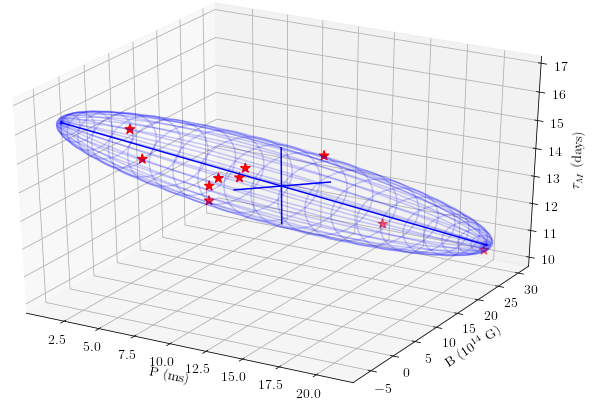
\includegraphics[width=\columnwidth]{./Original_3D_param_space.png}
    \caption{The $\tau_{M}$-B$_{14}$-P$_{ms}$ magnetar parameter space determined for our low-$z$ SLSNe sample. \angus{Need to find way to block out unphysical values in mesh plot!}}
    \label{fig:param_space}
\end{figure}

We test how representative this model parameter space is of the PTF sample of SLSNe-I within this redshift range by fitting their available photometry with the same magnetar model. We find that $\sim 75\%$ of the derived properties of the low-redshift PTF SLSNe-I fall within 3$\sigma$ of this model parameter space. We thus create a library of template PTF $R$-band light curves using the possible magnetars contained within this defined parameter space. We assume a UV absorbed black body as the underlying SED, and generate observer-frame light curves over all redshifts within the range 0.001$< z <$0.2, using a redshift bin size of 0.001.


\section{The Supernova Sample}

This section details the construction of both our CCSN and SLSN sample. Our primary obstacle is the classification of transients into the relevant sub-types. To alleviate this our sub-survey parameters were designed to encapsulate times when PTF achieved a regular cadence and high spectroscopic classification efficiency.  to minimise the misclassification of SNe and hence contaminants in the final sample. We first describe our light curve coverage cuts and discuss the details of our search for both spectroscopically confirmed as photometrically identified candidates. Again, we stress that any cuts we enforce our real SNe must also be applied to simulated objects later in the analysis.

\subsection{Light-curve coverage cuts}
\label{sec:coverage_cuts}

The cuts described here are primarily designed to maximise the probability that PTF would have spectroscopically classified the transient. In this regard, we adopt some of the choices made by \citet{Frohmaier19} in their construction of a SN Ia sample. Our coverage cuts are:

\begin{itemize}
    \item There must be at least four epochs on which the supernova is detected across the sub-surveys;
    \item An object is considered detected if the RB score $\ge$0.07 \citep{Bloom2012};
    \item These four epochs must be separated by $\ge$12 h;
\end{itemize}

These cuts were applied to  the real-time difference-imaging photometry\footnote{We searched an internal PTF light curve database. A publicly avaliable replica database, containing sources and photometry, can be accessed from \url{https://irsa.ipac.caltech.edu/} } obtained during the PTF survey operation and formed the foundation of our spectroscopic and photometric search for objects.

\subsection{The core-collapse sample}
\label{sec:CCSample}

We now turn our attention to the construction of the CCSN sample. Our first decision was to set a maxium redshift for an object to be included in our sample. This was set at z${\le}$0.035 and was motivated by ensuring that, at this distance, the fainter end of the CCSN luminosity function \chris{Put a citation: Li 2011} was above the detection limit of PTF (m ${\sim}$21.5). We then defined the sky area and date range over which to perform a search of real CCSNe. It is this part of the analysis where PTF presents itself as one of the more unique supernova hunting experiments. Other surveys, such as SDSS-SN \chris{cite SDSS}, \chris{SNLS}, or \chris{DES}, typically adopt a supernova observing strategy involving regular cadenced imaging of a fixed area of the sky. This naturally sets the survey volume for the supernovae, and consequently provides the boundaries for any simulations that aim to replicate the survey operation. PTF was different and performed an evolving search strategy that changed through the lifetime of the survey. To alleviate the complications of searching and simulating a varying footprint, we established 9 areas across 2010--2012 that PTF regularly observed so that we could model each as a distinct sub-survey. These areas were selected through a visual inspection of the PTF fields and were unbiased by the SN distribution on the sky. The parameterization of our sub-survey footprints are listed in Table XX and visualized in Figure XX. We then searched the PTF data to find SN candidates within these sub-surveys and we present our findings in the following sections.

\subsubsection{Spectroscopically confirmed CCSN}
\label{sec:spec_CC}

The spectroscopic follow-up campaign for the PTF survey was performed at several facilities and on a range of instruments. The majority of spectra were taken with the Double Spectrograph on the Palomar 200 inch telescope \chris{cite Oke and gunn 82}, the Keck 10 m telescope using the Low-resolution Imaging Spectrometer \chris{cite LIRS; Oke 1995}, the ISIS spectrograph on the 4.2 m William Herschel Telescope, and the Lick Observatory Shane 3 m telescope with the Kast souble spectrograph \chris{Mill and Stone 1993}.

Events were classified shortly after spectra were obtained using both visual inspection and through the automated classifers SNID \chris{Blondin 2007} and Superfit \chris{Howell 2005}. Core-collapse SNe were classified into their various sub-types based on their prominent spectral features (for an overview see; \chris{Fillipenko 1997?}); Type II (strong H lines), IIb (strong H and He lines), IIn (narrow H), Ib (no H, strong He lines), and Ic (no H or He lines). Additionally, events were classified as SN Ic-BL based on their similarities to, namely, SN 1998bw and SN 2002ap. Furthermore, our Type II events were not sub-divided further into light curve evolution driven categories (IIP/L groups), although we do distinguish Type IIb events as they are believed to originate from a stripped progenitor \chris{e.g. Chornock 2010, find more}.

We collated a sample of spectroscopically confirmed objects that met our spectroscopic definition of a CCSN, were detected in our sub-surveys, and passed the minimum light curve coverage cuts. In total we found 84 SNe (60 Type II, 24 SESNe) and present these objects in Table XX.


\subsubsection{Photometrically Identified CCSNe}
\label{sec:photCC}

Due to the limited spectroscopic follow-up resources avaliable to any sky survey, it is enevitable that some SNe will only be identifable through their photometric evolution. Finding these missed events required a search of the PTF transient data base containing $\sim 48 000$ unique candidate objects. This database not only contains SNe, but also a variety of other transient phenomena, such as variable stars and activatae galatic nuclei. Additionally, a large contaminant of non-atrophysical events comes from spurious detections caused by subtraction artefacts.

We begin by applying our strict light curve quality cuts from Section~\ref{sec:coverage_cuts} and sub-survey parameters from TableXX to reduce the number of potential PTF SN candidates to 987. Most of these objects, however, have been spectroscopically typed and removing those with a definitive classification reduces our candidate sample size to 20. We note that if the object was spectroscopically observed and the classification was unclear we retained the object in our prelimnary sample. These final candidates were cross matched to the SDSS galaxy catalogues and visually inspected to confirm no host misidentification \chris{cite sullivan and gupta} and in the event of a galaxy redshift we rejected objects with $\mathrm{z}_\mathrm{host}{>}0.035$. This resulted in three objects that warranted further investigation; PTF12bvf, PTF12cxz, PTF12gfx. We were able to cross-match PTF12cxz with a known SN-imposter candidate which was later identified in 2014 \citep{2014ATel.5737....1T}, we thus conclude that PTF12cxz is was likely a luminous blue variable eruption and can be excluded from out sample.

Our final candidates, PTF12bvf and PTF12gfx, are presented in Table~\ref{tab:photCCproperties} and both have host spectroscopic redshifts that fall within our sample requirements. We thus consider these objects to be viable CCSN candidates and include them in the rates analysis in SectionXX.

\begin{table}
    \caption{PTF CCSN photometric candidates }
    \centering
    \chris{CHRIS, put the goddam coordinates in sexagesimal and add ALL CC candidates}\\
	\begin{tabular}{l l l l l l} 
		\hline

ptfname &     ra     &    dec     & redshift  \\
		\hline
 PTF12bvf   &  177.75691 &  20.399901 & 0.022  \\
 PTF12gfx   & 240.413968 &  16.310245 &    0.029 \\
 
 		\hline
		\label{tab:photCCproperties}
	\end{tabular}
 \end{table}


\subsection{The SLSN sample}
\label{SLSN_sample}

The PTF hydrogen-poor SLSNe we consider for this rates analysis were classified in \chris{Quimby 2018} and the light curves were presented in \chris{De Cia}. In total, 26 SLSNe-I were studied from PTF and iPTF to form the largest low-redshift, homogeneously selected, sample of SLSN-I to-date. The host galaxies of the PTF SLSN sample are presented in \chris{Perely}, however their sample differs slightly to other PTF analyses due to a different sample luminosity cut. 

We choose to draw our candidates from TableXX in \chris{De Cia} and subsequently obtained their light curves from the PTF transient data base. Each light curve was then checked to see if it met the coverage cuts described in Section~\ref{sec:coverage_cuts}. We are presented with a choice of redshift cut at this stage of the analysis which, again, is motivated by a desire to have a high sample completeness. The volume weighted mean redshift of the \chris{De Cia} sample is $\langle \mathrm{z} \rangle = 0.33$ and they claim the redshift distribution monotonically falls beyond z${\sim}$0.5 due to an observational bias set by by the limiting magnitude of the PTF survey. Undeniably, all surveys are affected by a malmquist bias, however, given the uncertainties in the SLSNe-I luminosty function and the small number of events driving the redshift distribution, we choose to be conservative in our rate sample redshift limit and set it to be z${\le}$0.2. This limit coincides with an apparent peak in the \chris{De Cia} redshift distribution and also ensures the the majority of objects simulated from our own luminosity function in SectionXX \chris{SLSN-Templates} will be detectable by PTF. Applying this redshift cut to the \chris{De Cia} sample provides us with 8 objects.

Talk about how this is whole sky


\subsection{Host Surface Brightness}
\label{sec:fox_distribution}

Talk about fbox here, but go home now chris.


\section{Rate Simulation and Results}
\label{sec:rate_sim}

In this section we detail the process of calculating the CCSN and SLSN-I rates from the PTF data. We follow the methodology principles laid out in Section~\ref{sec:ratesPTF} and describe the subtle differences in the treatment of data for the each of our calculated rates. We also present the measurement uncertainties and justfiy how our method naturally incorporates the statistical and systematic uncertainties into a single probability density function. We begin by calculating the rate of CCSNe and follow this by extracting only the SESNe for a seperate analyses. We then perform a near identical study on the SLSNe-I and conclude by comparing all sub-sets to investigate the relative fractions.

\subsection{Core-Collpase Supernova Rate}
\label{sec:CCSN_Rate}

Our calculation of the volumetric rate begins with a large Monte Carlo simulation where many realizations of an intrinsic SN rate, $r_\mathrm{intrinsic}$, are drawn along with the fixed $T_\mathrm{obs}$ and $V_\mathrm{obs}$ for the sub-surveys. These values are used in Equation~\ref{eqn:poiSim} to generate an $N_\mathrm{input}$ and, following the methods in Section~\ref{sec:ratesPTF}, a subsequent value of $N_\mathrm{output}$ is determined. This process was repeated for 400 000 realizations of the intrinsic CCSN rate, $r_\mathrm{intrinsic}$, to produce a corresponding set of $N_\mathrm{output}$. At this stage, it is possible to trace any value of $N_\mathrm{output}$ to analyse the distribution of initial $r_\mathrm{intrinsic}$ \citep[e.g.][]{Prajs2016}, however, our story is not yet complete as we must also include an uncertainty on our true SN sample size.

The CCSN sample consists of 86 candidate events that were discovered in our previously described sub-surveys and passed our strict observational cuts. The observed number of SN events follows an intrinsic rate (for any given volume and time-span) that is governed by the statistics of the Poisson point-process. The probability of observing an integer $n$ events given we have $N_\mathrm{obs}=86$ observed events follows the Poisson distribution, identical in functional form to Equation~\ref{eqn:poiSim} 

\begin{equation}
    P(n; N_\mathrm{obs})=\frac{N_\mathrm{obs}^{n} e^{-N_\mathrm{obs}}}{n!}
    \label{eqn:poiObs}
\end{equation}
\chris{I think $N_\mathrm{obs}^{n}$ looks messey, how else should we present it?}
In principle, n extends over the range $0 \le n \le \infty$, however, in practise $P(n=N_\mathrm{obs}$ quickly becomes vanishingly small either side of the maximum probability for our sample size of $N_\mathrm{obs}=86$. We, therefore, only compute the probabilities over a finte range of n where beyond this the probabilites have a negliable effect on the final result.

We now infer our final rate by bootstrap sampling from Equation~\ref{eqn:poiObs} and couple this with the output of the rate simulations. Firstly, we sample a value of $n$ from Equation~\ref{eqn:poiObs} to set the observed number of events for our trial. We then compare all outputs from the rate realizations described in Section~\ref{sec:ratesPTF} where $N_\mathrm{output} =  n$ to form a set of corresponding intrinsic rates $r_\mathrm{intrinsic}$. We then randomly select a value from this set to assume the instrinsic CCSNe rate for this realization. This process was repeated many tens of thousands of times to build up a distribution of $r_\mathrm{intrinsic}$ which we present in Figure~\ref{fig:ccRateDist}. A skewed Gaussian was then fit to this distribution to find the peak of the distribution and the $1\sigma$ uncertainties - calculated as the interval containing 68.3 per cent of the probability around the mean. We, therefore, infer the volumetric rate of CCSNe to be $r^\mathrm{CC}_v=9.10_{-1.27}^{+1.55}\times10^{-5}\,\text{SNe yr}^{-1}\,\text{Mpc}^{-3}\, h_{70}^{3}$ at the simulated sample volume-weighted mean redshift of $ \langle z \rangle = 0.028$.

\begin{figure}
	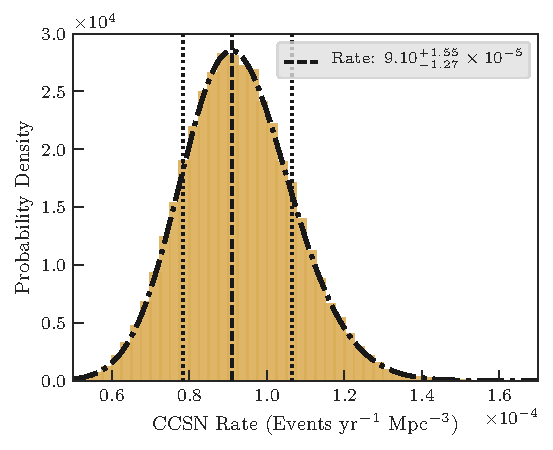
\includegraphics[width=\linewidth]{./allCC_Rate.pdf}
    \caption{The intrinsic CCSN rate distribution.}
    \label{fig:ccRateDist}
\end{figure}


\subsubsection{Stripped-envelope supernova rate}
\label{SESN_Rate}

We now shift our focus to a subset of the CCSN sample and look to apply our rate methodology to the SESNe. Our sample consists of 24 spectroscopically confirmed objects listed in TableXX. Once again we must include our contamimnant supernovae of unknown type, PTF12bvf and PTF12gfk, as a systematic uncertainty in the final estimate of our rate. This brings our total sample size to 26 SESNe and we use this number as our $N_\mathrm{obs}$ in Equation~\ref{eqn:poiObs} and follow the prescription of Section~\ref{sec:CCSN_Rate}. It is worth empahsising that this measurement of the SESN rate is performed completely independently of the CCSN simulation and is, therefore, unaffected by any assumptions on the SESN to CCSN population fraction. We performed another 400,000 realizations of just the SESN rate to probe the intrinsic SESN rate related to discovering 26 events. The probability distribution is presented in Figure~\ref{fig:SESNrateProbDist} and shows that the most likely SESN rate is $r^\mathrm{SE}_v=2.41_{-0.64}^{+0.88}\times10^{-5}\,\text{SNe yr}^{-1}\,\text{Mpc}^{-3}\, h_{70}^{3}$ at a volume weighted mean redshift of $ \langle z \rangle = 0.028$.

\begin{figure}
	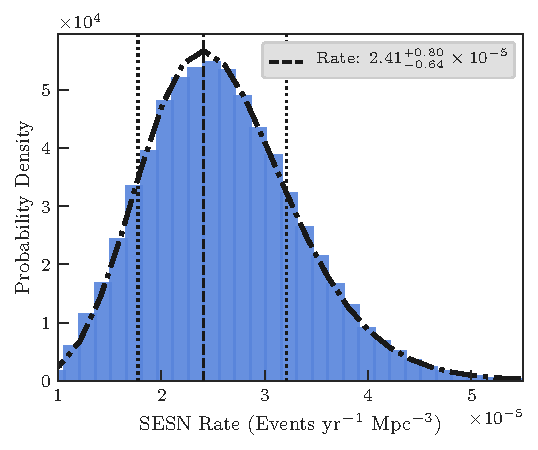
\includegraphics[width=\linewidth]{./SESN_Rate.pdf}
    \caption{The SESN rate probability distribution}
    \label{fig:SESNrateProbDist}
\end{figure}

\subsection{Comparison to literature rates}

We now compare our CCSN rates to those from other surveys at low-redshift ($z<0.4$). We select works that have computed volumetric rates directly from rolling search data \citep[e.g.][]{2009A&A...499..653B}, or from those that have converted rates in units of host-galaxy properties to volumetric rates following \citet{2008A&A...479...49B}. Our curated sample of 8 CCSN rate measurments spans the range $0\lesssim z \lesssim 0.4$ and is presented in Figure~\ref{fig:rates_CC_lit}, where relevant the measurements have been corrected to our cosmology. Furthermore, we do not discriminate between rates calculated from rolling surveys \citep[e.g.][]{2009A&A...499..653B} and galaxy targetted surveys \citep[e.g.][]{1999A&A...351..459C}.

\begin{figure*}
	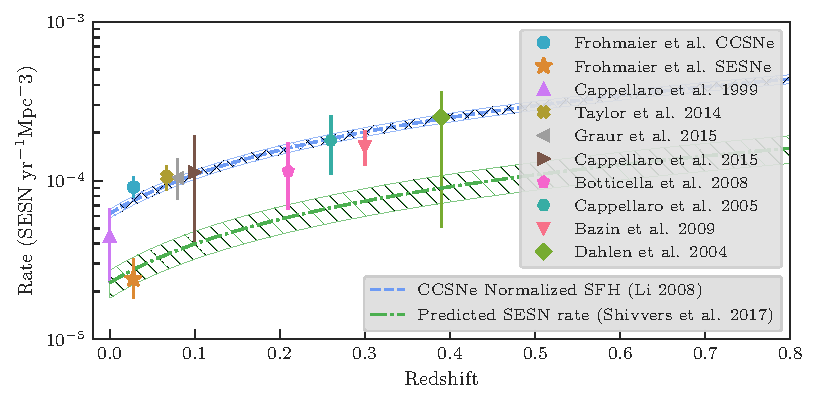
\includegraphics[width=\linewidth]{./allCC_Compare_Literature.pdf}
    \caption{The volumetric CCSN rate evolution as function of redshift compared to measurements from the literature \citep{1999A&A...351..459C,2014ApJ...792..135T,2015MNRAS.450..905G,2015A&A...584A..62C,2008A&A...479...49B,2005A&A...430...83C,2009A&A...499..653B,2012ApJ...757...70D}. We fit a normalised SFH history \citep[blue dashed line;][]{2008MNRAS.388.1487L} to the CCSN rate sample and represent our $1\sigma$ uncertainties with the hatched region. Our measurement of the SESN rate is represented by the orange star, the SFH history we fit to the CCSN sample is scaled according to the relavtive population fractions of SESNe/CCSNe from \citet{2017PASP..129e4201S}, and is represented by the green dot-dashed line.}
    \label{fig:rates_CC_lit}
\end{figure*}

We now briefly summarise the comparable rate measurments through increasing redshift. The CC rate measurement of \citet{1999A&A...351..459C} was constructed by collecting data from several different SN surveys, including a visual search for local supernovae, and presented as a function of host galaxy properties. This result was converted to a volumetric rate following \citet{2008A&A...479...49B} and found to be $0.43\pm 0.17 \times10^{-4}\,\text{SNe yr}^{-1}\,\text{Mpc}^{-3}\, h_{70}^{3} $ at $z=0.01$. The CCSN rate of \citet{2014ApJ...792..135T} was calculated from 89 CCSNe in the Sloan Digital Sky Survey \citep[SDSS;][]{2000AJ....120.1579Y,2011AJ....142...72E} photometric search for SNe, they found a CCSNe rate of $1.06\pm 0.19 \times10^{-4}\,\text{SNe yr}^{-1}\,\text{Mpc}^{-3}\, h_{70}^{3} $, $z=0.072$. This contrasts to the rate of \citet{2015MNRAS.450..905G} who searched for contaminant SN flux in SDSS galaxy spectra to obtain a rate of $1.04_{-0.26}^{+0.33}\mathrm{(stat)}_{-0.11}^{+0.04}\mathrm{(sys)} \times10^{-4}\,\text{SNe yr}^{-1}\,\text{Mpc}^{-3}\, h_{70}^{3} $, $z=0.075$, from a sample of 16 CCSNe. The Supernova Diversity and Rate Evolution \citep[SUDARE;][]{2013Msngr.151...29B} performed a search for SNe at intermediate redshifts and found 50 CCSNe and measure the rate to be $1.13_{-0.53}^{+0.62}\mathrm{(stat)}_\pm 0.49\mathrm{(sys)} \times10^{-4}\,\text{SNe yr}^{-1}\,\text{Mpc}^{-3}\, h_{70}^{3} $, $z=0.1$. We now jump in redshift to $z=0.21$ where a galaxy targetted search for supernovae was performed by STRESS and presented the CCSN rate $1.15_{-0.33}^{+0.43}\mathrm{(stat)}_{-0.36}^{+0.42}\mathrm{(sys)} \times10^{-4}\,\text{SNe yr}^{-1}\,\text{Mpc}^{-3}\, h_{70}^{3} $ from a weighted sample of 44.95 objects \citep{2008A&A...479...49B}. Using the cosmic SFR and the galaxy luminosity density, \citet{2005A&A...430...83C} converted their galaxy targeted rate into a volumetric rate to find $2.2_{-0.7}^{+0.8} \times10^{-4}\,\text{SNe yr}^{-1}\,\text{Mpc}^{-3}\, h_{75}^{3} $, $z=0.26$. The largest sample size in our literature compilation, with N=117 CCSN, comes from the Supernova Legacy Survey (SNLS) \citep{2009A&A...499..653B} rolling search with candidates out to redshifts $z<0.4$. They measure the CCSN rate to be $1.42 \pm 0.3 \mathrm{(stat)} \pm 0.3 \mathrm{(sys)} \times10^{-4}\,\text{SNe yr}^{-1}\,\text{Mpc}^{-3}\, h_{70}^{3}$ at $z=0.3$. Finally, we include the rate measurement of \citet{2012ApJ...757...70D} from a sample of 9 CCSNe in their lowest-redshift bin ($z=0.39$) from Hubble Space Telescope data following a Monte Carlo simulation similar in concept to our own and described in \citet{2004ApJ...613..189D}. They find a CCSN rate of $3.00_{-0.94}^{+1.28}\mathrm{(stat)}_{-0.57}^{+1.04}\mathrm{(sys)} \times10^{-4}\,\text{SNe yr}^{-1}\,\text{Mpc}^{-3}\, h_{70}^{3} $.

The literature sample, including our own CCSN and SESN rate measurements, are presented in Figure~\ref{fig:rates_CC_lit} and illustrates that the CCSN rate increases with redshift. This reflects the increasing SFR with look back time due to CCSNe exploding relatively promptly after formation ($\lesssim40\,\mathrm{Myr}$). We normalised the cosmic Star Formation History (SFH) as parameterised by \citet{2008MNRAS.388.1487L} with the \citet{2001MNRAS.326..255C} functional form. This is presented in Figure~\ref{fig:rates_CC_lit} by the blue dashed line. Assuming the CCSN rate follows this simple evolution from z=0 over a look back time of $\sim4.3$Gyr, we find the CCSN rate increases by a factor of $\sim 4.2$.

We are unable to make any assertions on the fraction of CCSN that are SESNe from our data as this ratio is an implicit assumption used in the CCSN rate simulation. However, we can use the \citet{2017PASP..129e4201S} population fractions to probe any systematic biases in our simulation pipeline. It is natural to expect that the brighter intrinsic luminosities of SESNe would make them easy to discover and, hence, introduce a malmquist bias. We explored this by taking our normalised SFH and scaling it by the estimated SESN population fractions. This is presented in Figure~\ref{fig:rates_CC_lit} by green dot-dashed line and is in good agreement with our measured SESN rate represented by the orange star. We are, therefore, confident that our rate simulations are unaffected by the malmquist bias and futher adds credence to our independent measurement of the absolute SESN rate.


\section{SLSN-I Rate}

We now examine the rate of SLSNe-I from our PTF data. Chris needs to write this asap!


\begin{figure*}
	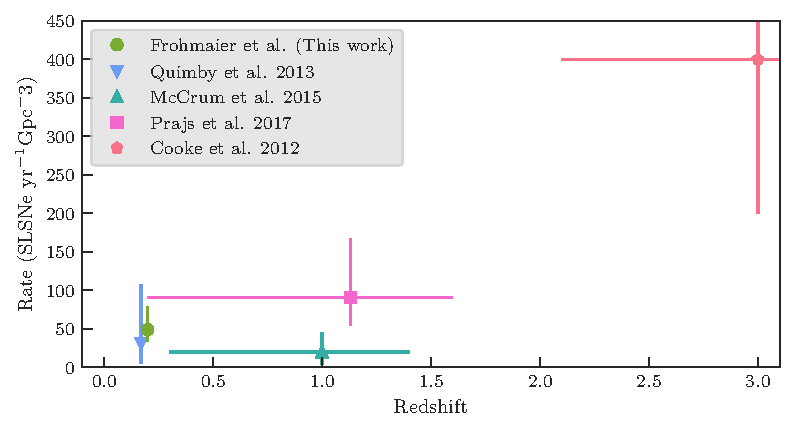
\includegraphics[width=\linewidth]{./SLSN_Compare_Literature.pdf}
    \caption{}
    \label{fig:rates_SLSN_Lit}
\end{figure*}

% In this Section we describe our method of calculating the SLSN-I rate in the PTF data. The complexities of calculating supernova rates in survey data are amplified in PTF due to the large observing footprint, variable cadence, and rarity of SLSN-I. To calculate the rate we considered adopting an ``efficiency weighting'' approach \citep[e.g.][]{Perrett12, Frohmaier19} where individual objects are weighted according to the results of a survey simulation. Whilst this method was effective at calculating the SN Ia rate in PTF, \citet{Frohmaier19} required strict data quality cuts in a regularly cadenced domain that only a sub-set of SNe Ia met (N=90). This methodology was justified as it reduced the systematic uncertainties associated with poor quality data, without sacrificing much of the statistical relevance of their sample size. This is something we are unwilling to do as our SLSN-I sample is small to begin with.

% We, therefore, adopt and extend a Monte-Carlo simulation approach, similar to \citet{Prajs2016} and \citet{Frohmaier18}, to estimate the SLSN-I rate. Within the Monte-Carlo simulation an intrinsic volumetric rate ($r_\mathrm{intrinsic}$) is assumed and used to calculate the number of template light curves to enter the simulation. The template properties are drawn from the input parameter distributions described in Section~\ref{fig:param_space}. We then trial different values of $r_\mathrm{intrinsic}$ to build a probability distribution of cases when the simulation output sample is equal in size to the PTF observed sample size ($N_\mathrm{output}=N_\mathrm{observed}$).

% When calculating any rate, careful consideration must be taken to account for observational biases within the simulation. Our observational detection efficiencies are taken from \citet{Frohmaier17}. As part of the analysis around 7 million artificial point sources were inserted into real observations, this characterised the PTF transient detection pipeline as a function of several key observational properties (source magnitude, seeing, sky background, limiting magnitude, host surface brightness). Ultimately, these detection efficiencies describe the probability that, on any given night during the survey, PTF would have detected an event.

% Building on these principles, our method for calculating the volumetric SLSN-I rate proceeds as follows. We first define the sky area and redshift range over  which PTF would have been sensitive to SLSNe. Unlike other PTF rates analyses \citep{Frohmaier18, Frohmaier19}, we do not sub-divide the sky into smaller well-controlled `sub-surveys' with a regular cadence. This is because the long duration of SLSN light curves makes them less susceptible to cadence variations. We, therefore, simulate SLSNe over a ${\sim}$30,000\,deg$^2$ total footprint ($\Theta_\mathrm{obs}$) \chris{(The 30,000deg simulation is `id=2' in the database)}\ across 3 years of operation from 2010--2012 ($T_\mathrm{obs}$). We are unable to perform light curve simulations in data taken in 2009 due to the unreliable nature of the recovery efficiencies during the survey's first few months of operation. We set the upper limit for a simulated object to be z=0.2 following our sample definition in Section~\chris{Write about the sample}.






In this Section we present the SLSN-I volumteric rate and discuss the associated uncertainties with this result. The small size of our SLSN sample (N=10) necessarily dictates that our final result is statistics limited. The advantage of our Monte-Carlo simulation technique is the intuitive interpretation of our uncertainties \angus{Humble brag alert}.

We first generate a probability density function (PDF) for the rates that produced $N_\mathrm{observed}=10$ observed SLSNe. This is not the final probability distribution as the number of SNe occurring in a given time-span is described by a Poisson process. To capture this natural variation in counting statistics we weight subsequent PDFs assuming $N_\mathrm{observed}=(0, 1, 2, \dots)$ following 
\begin{equation}
    \omega_i(i; \lambda=10)=e^{-\lambda }{\frac {\lambda ^{i}}{i!}} \mathrm{~for~} i=0, 1, 2, \dots
\end{equation}

where $\omega_\mathrm{i}$ is the weight factor, i is the number of SNe observed, and $\lambda$ is the most probable value. 

\comment{\chris{Chris to finish....}}


We measure a final rate of 49$^{+28}_{-18}$ SLSN-I events yr$^{-1}$ Gpc$^{-3}$ at $z=0.2$. This is consistent with the measurement of \citep{Quimby2013} at similar redshift ($z=0.17$). In Fig. \ref{fig:rates_SLSN_Lit}, we compare the PTF SLSN rate measurement with other published values taken from the literature (e.g. \citep{Quimby2013,McCrum2015,Prajs2016,Cooke2012}) 
%as a function of redshift alongside the cosmic star-formation history normalised to our well-constrained PTF SLSN rate measurement \citep[SFH; see][]{Hopkins2006}. As expected from progenitor models, the evolution of the SLSNe rate roughly traces the evolution of star-formation throughout cosmic time, although alone this evolution is not enough to distinguish between progenitor masses beyond the $\sim$8 M$_{\odot}$ progenitor divide between thermonuclear and core-collapse progenitors.


SLSNe-I are intrinsically rare events, with an estimated rate of 0.001\% of the core-collapse SN (CCSN) rate in the local Universe \citep{Quimby2011,Quimby2013,McCrum2015}, which ostensibly increases with redshift, following trends in the cosmic star formation history \citep{Prajs2016,Cooke2012,Moriya2018}. 


The majority of models for SLSN production reply upon the collapse of single, massive stars, although exactly how massive these progenitors need to be is still uncertain. Even within particular explosion paradigms, the mass of the progenitor can vary as a result of subtle tweaks in the pre-explosion assumptions \comment{\angus{CITE SOME SHIT!}}. Furthermore, the driving environmental properties attributed to the production of a SLSN progenitor over that another core collapse event are difficult to disentangle, be it low-metallicity environments or intensley star forming regions. This is particularly difficult to do in the low-redshift Universie (where the majority of SLSN hosts have identified and studied), as the majority of cosmic star formation in the local Universe is tied up in small, low mass star-bursting galaxies \comment{\angus{REFS}}. 

Rates provide one way in which we can break the degeneracy between host star formation properties and metallicity. By comparing the ratio of rates of SLSNe to those of other core collapse transients across different redshifts (under the assumption of a constant IMF), we may begin to establish whether any evolution in this ratio is reflected in global galaxy evolution properties (such as the evolution of mass/metallcity with redshift).  \angus{{\bf{To test this, we estimate the rate of all stripped-envelope SNe (SESNe) in PTF using the templates of Vincenzi et al 2019.}}}

\section{Summary}


\begin{figure}
	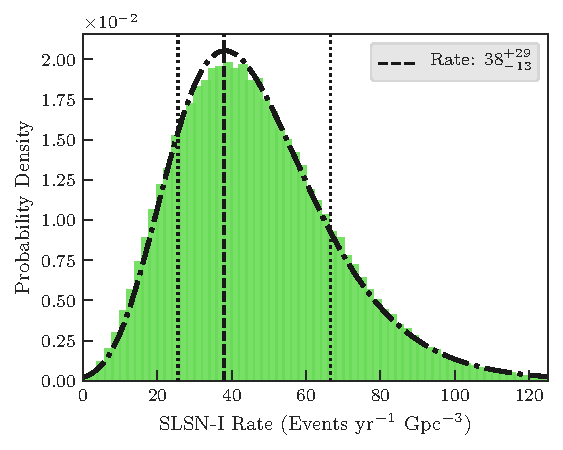
\includegraphics[width=\linewidth]{./SLSN_Rate_Dist.pdf}
    \caption{The SLSN-I rate probability distribution}
    \label{fig:SLSNrateProbDist}
\end{figure}



% \begin{figure}
% 	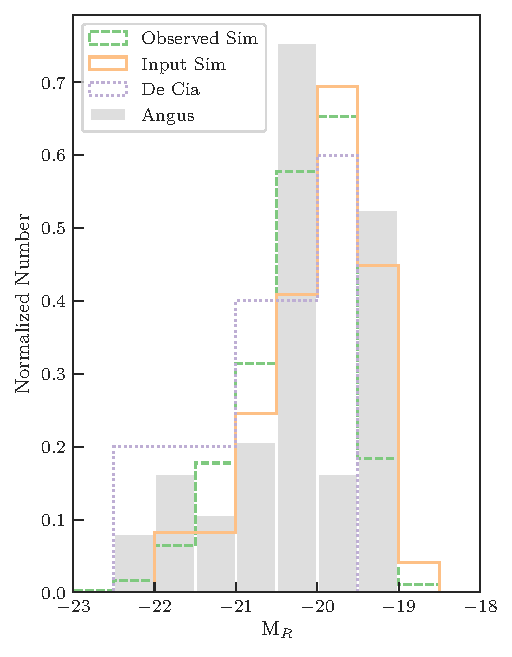
\includegraphics[width=\linewidth]{./ObservedLF_compare.pdf}
%     \caption{}
%     \label{fig:lum_func}
% \end{figure}
\section{Summary}


\begin{figure}
	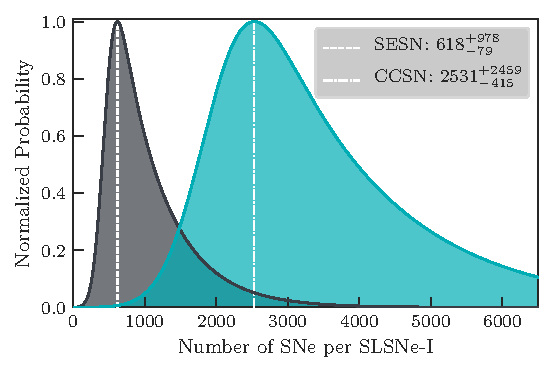
\includegraphics[width=\linewidth]{./bothRateCompare.pdf}
    \caption{The SLSN-I rate probability distribution}
    \label{fig:compare2SLSN}
\end{figure}

\section*{Acknowledgements}


%%%%%%%%%%%%%%%%%%%%%%%%%%%%%%%%%%%%%%%%%%%%%%%%%%

%%%%%%%%%%%%%%%%%%%% REFERENCES %%%%%%%%%%%%%%%%%%

% The best way to enter references is to use BibTeX:

% \bibliographystyle{mnras}
% \bibliography{references} % if your bibtex file is called example.bib


% Alternatively you could enter them by hand, like this:
% This method is tedious and prone to error if you have lots of references

\bibliographystyle{mnras}
\bibliography{references} 
%%%%%%%%%%%%%%%%%%%%%%%%%%%%%%%%%%%%%%%%%%%%%%%%%%

%%%%%%%%%%%%%%%%% APPENDICES %%%%%%%%%%%%%%%%%%%%%

\appendix

\section{Some extra material}

If you want to present additional material which would interrupt the flow of the main paper,
it can be placed in an Appendix which appears after the list of references.

%%%%%%%%%%%%%%%%%%%%%%%%%%%%%%%%%%%%%%%%%%%%%%%%%%


% Don't change these lines
\bsp	% typesetting comment
\label{lastpage}
\end{document}

% End of mnras_template.tex